\documentclass[11pt,a4j,twocolumn]{jarticle}
\usepackage{csbstp}
\usepackage{amsmath}
\usepackage[dvipdfmx]{graphicx}
\usepackage{amssymb}
\usepackage{algorithm}
\usepackage{algorithmic}
\usepackage{subcaption}
\usepackage[dvipdfmx]{color}

\def\AgentSet{A}
\def\Dreq{{D_{\it req}}}
\def\En{\mathcal{E}}
\def\SelfAss{{S_{\it ass}}}

\def\BatteryMax{{B_{\it max}}}
\def\BatteryLevel{b}

\def\HomingCheck{{T_{\it homing}}}
\def\HomingBattery{{k_{\it homing}}}
\def\PausingInt{{S_{\it pause}}}

\def\PauseTimeFactor{{\gamma_{\it p}}}

\def\DeactCheckStartTime{D_{\it st}}
\def\DeactCheckInterval{D_{\it int}}
\def\PauseCount{x_{\it pause}}
\def\DeactCount{N_{\it deact}}
\def\DeactThreshold{K_{\it deact}}
\def\DeactLearnInterval{D_{\it learn}}


\title{マルチエージェント協調巡回問題におけるエネルギー消費抑制手法の提案}
\author{松本~航平}
\studentid{1W193102}
\university{早稲田大学}
\faculty{基幹理工学部}
\department{情報理工学科}
\advisor{菅原~俊治}
\type{卒業論文}
\nendo{2022}
\hizuke{\today}

\begin{document}
\maketitle
\section{序論}
近年,ロボット技術が発達し,巡回パトロールや清掃などといった,人間が日常的に繰り返す作業を
複数の自律ロボットで代替する動きが加速している.
このような複数のロボットが協調して共通の作業を行う問題は,
マルチエージェント協調巡回問題(MACPP)と呼ばれる.
この研究では,複数のエージェントが協力・協調することで,
与えられた環境で効率的に巡回を行うことを目的としている.
\par

巡回効率だけを追求した高度な行動や学習は,確かに巡回の効率は向上するものの,
必要以上にエネルギーを消費する可能性がある.
一方,アプリケーションによっては,巡回作業に対する品質要求があり,
それを超えることは必ずしも期待されているわけではない.
例えば清掃問題では,ある程度環境がきれいになっていれば十分であり,
過度の巡回作業はかえって単位エネルギー当たりの作業効率を低下させる.
\par

MACPPにおいてエネルギー効率に注目した研究として\cite{Wu2019}がある.
\cite{Wu2019}では,エージェントが要求を満たせば自律的に充電基地への帰還({\em Homing})や,
充電基地での待機({\em Pausing})を行い,エネルギーを節約する手法を提案している,
本研究では,\cite{Wu2019}の手法を拡張し,
その後の行動によって起こりうる貢献を自律的に予測し,
環境の現状を推定することで品質要求の全体的な達成度を把握しながら,
品質要求の充足とエネルギー消費の削減を両立する手法を提案する.

\section{モデルの定義}
\subsection{環境}
エージェントの巡回環境をグラフ$G = (V,E)$で表す.
ここで,$V = \{v_1, \dots, v_n \}$はノード集合を表し,
各ノード乗にエージェントやイベント,障害物が存在する.
また,$E$はノード$v_i$と$v_j$間のエッジ$e_{i,j}$である.
本研究では,エッジの長さはすべて1とする.
さらに,ステップを単位とする離散時間を導入する.
したがって,エージェントは1ステップで障害物のない隣接ノードに移動することができる.
\par

全てのノード$v\in V$上でイベントが発生し,そのイベント発生確率を$p(v)~(0\leq p(v)\leq 1)$とする.
毎時刻$t$において,ノード$v$に蓄積されたイベント数$L_t(v)$は以下の式で更新される.
%
\begin{equation}
  L_t(v) = \left\{
\begin{array}{ll}
  L_{t-1}(v) + 1 & \textrm{(確率$p(v)$のイベント発生時)} \\
  L_{t-1}(v) & \textrm{(その他)}
\end{array}
\right.  
\end{equation}
%
時刻$t$にエージェントがノード$v$を訪れた時に$v$上のイベントは処理され,$L_t(v) = 0$となる.

\subsection{エージェント}
$n$個のエージェントの集合を$\AgentSet=\{1,\dots ,n\}$と表す.
エージェント$i\in\AgentSet$はバッテリを持ち,バッテリ容量が0になる前に充電基地に戻り充電し,
完了後は再び環境を巡回する.
\par

エージェントは目標決定戦略によって,目標ノード$v^i_{tar}$を決定する.
その後,経路生成戦略によって,$v^i_{tar}$までの経路を生成し,
それに沿って行動を進める.
これをバッテリ残量を参照しながら繰り返す.

\subsection{評価指標}
本研究では評価指標として以下の式で定められるイベント残存時間の総和$D_{t_s,t_e}$と,
エージェントの総エネルギー消費量$C_{t_s,t_e}$を用いる.
%
\begin{align}
  D_{t_s,t_e} &= \sum_{v \in V} \sum^{t_e}_{t=t_s+1} L_t(v)\\
  C_{t_s,t_e} &= \sum_{i \in \AgentSet} \sum^{t_e}_{t=t_s+1} \En_t(i),
\end{align}
%
ここで,$[t_s,t_e]~(t_s < t_e)$ は時間間隔を表し,
$\En_t(i)$は$t$におけるエージェント$i$の消費エネルギーを表す.
したがって,$i$が隣接ノードに移動したとき$\En_t(i)=1$,
それ以外は$\En_t(i)=0$となる.
\par
また,\cite{Wu2019}と同様に1stepにおけるイベント量の要求値$\Dreq$を設定した.
エージェントは以下の式を満たせるように協調を行う.
%
\begin{equation}\label{eq:condition}
  D_{t_s,t_e}\leq \Dreq \times (t_e - t_s)
\end{equation}
%
本研究では,品質要求(式(\ref{eq:condition}))を満たしつつ,$C_{t_s, t_e}$をできるだけ小さくすることが目的である.
以降,それぞれを$D(s), C(s)$と表す.


\section{提案手法}
本研究では,エージェントがそれぞれの視点で将来の環境状態を予測する方法を学習し,
充電基地についた際に,未来の環境状態を予測し,待機時間を動的に決定する手法として,AMTDS/ERを提案した.
\par

まず,エネルギー節約行動の調整のため,学習パラメータ$K^i$を$\forall i\in \AgentSet$に導入する.
{\em Pausing}後にイベント量の推定値$E^i(D_t)$を用いて$K^i$は個々に次の式に従って更新される.
%
\begin{equation}\label{eq:ParameterK}
  \begin{cases}
    K^i \gets (1 - \alpha_k) \cdot K^i + \alpha_k \cdot \dfrac{\Dreq}{E^i(D_t)}K^i 
    \hfill (E^i(D_t) \leq \Dreq)\\
    K^i \gets K^i - \left( \dfrac{E^i(D_t)}{\Dreq} - 1 \right) 
    \hfill (E^i(D_t) > \Dreq)
  \end{cases}
\end{equation}
%
次に,従来手法では{\em Pausing}は固定時間$\PausingInt$ステップしか待機しなかったが,
式(\ref{eq:revised})を満たす最大の$T (= \PauseTimeFactor\cdot\PausingInt)$まで待機するように変更した.
ここで,$t_c$は現在の時刻であり,$\PauseTimeFactor$は可変長の変数である.
さらに,{\em Homing}の後は必ず{\em Pausing}を行うようにした.
% 
\begin{equation}\label{eq:revised}
  \sum_{v \in V} E^i(L_{t_c+T}(v)) \div K^i \leq \Dreq
\end{equation} 
%

\begin{figure}
  \centering
  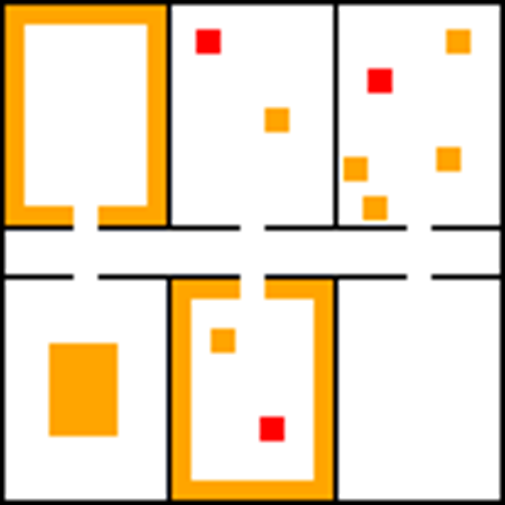
\includegraphics[width=0.5\hsize]{figures/Graph_Office.png}
  \caption{実験環境}
  \label{fig:env}
\end{figure}

\begin{figure}
  \centering
  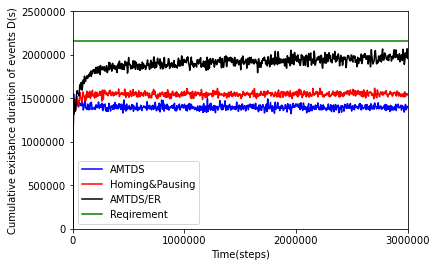
\includegraphics[width=0.8\hsize]{figures/ds_graph_3600_ave_ER_Office_600.png}
  \caption{$D(s)$の時間推移}
  \label{fig:ds_ER_Office}
\end{figure}

\begin{figure}
  \centering
  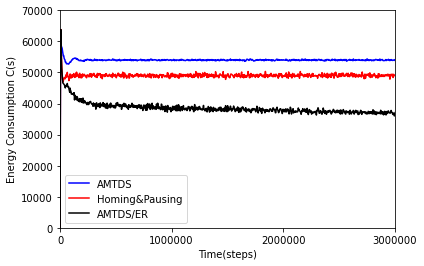
\includegraphics[width=0.8\hsize]{figures/cs_graph_3600_ave_ER_Office_600.png}
  \caption{$C(s)$の時間推移(実験1)}
  \label{fig:cs_ER_Office}
\end{figure}

\section{実験}
\section{結論}

\bibliographystyle{junsrt}
\bibliography{ref}
\end{document}